\documentclass[12pt,letterpaper]{exam}
\usepackage[lmargin=1in,rmargin=1in,tmargin=1in,bmargin=1in]{geometry}
\usepackage{../style/exams}

% -------------------
% Course & Exam Information
% -------------------
\newcommand{\course}{MAT 101: Exam 3}
\newcommand{\term}{Fall -- 2023}
\newcommand{\examdate}{12/13/2023}
\newcommand{\timelimit}{85 Minutes}

\setbool{hideans}{false} % Student: True; Instructor: False

% -------------------
% Content
% -------------------
\begin{document}

\examtitle
\instructions{Write your name on the appropriate line on the exam cover sheet. This exam contains \numpages\ pages (including this cover page) and \numquestions\ questions. Check that you have every page of the exam. Answer the questions in the spaces provided on the question sheets. Be sure to answer every part of each question and show all your work. If you run out of room for an answer, continue on the back of the page --- being sure to indicate the problem number.} 
\scores
\bottomline
\newpage

% ---------
% Questions
% ---------
\begin{questions}

% Question 1
\newpage
\question[10] Without using a calculator and showing all your work, solve the following system of equations:
	\[
	\begin{cases}
	4x + 2y= -4 \\
	6x - 5y= 18
	\end{cases}
	\] \pspace

\sol First, we shall solve this by substitution. We will solve for $y$ in the first equation. We have\dots
	\[
	\begin{gathered}
	4x + 2y = -4 \\
	2y = -4x - 4 \\
	y = -2x - 2
	\end{gathered}
	\]
We then use this in the second equation:
	\[
	\begin{gathered}
	6x - 5y = 18 \\
	6x - 5(-2x - 2) = 18 \\
	6x + 10x + 10 = 18 \\
	16x + 10 = 18 \\
	16x = 8 \\
	x = \frac{1}{2}
	\end{gathered}
	\]
But then $y = -2x - 2= -2 \cdot \frac{1}{2} - 2= -1 - 2= -3$. Therefore, the solution is $(\frac{1}{2}, -3)$. \pspace

Next, we solve the system using elimination. We shall eliminate $x$ from the system. We multiply the first equation by $3$ to obtain $12 + 6y = -12$ and the second equation by $-2$ to obtain $-12x + 10y = -36$. We then add these equations: \par
	\begin{table}[ht]
	\centering
	\begin{tabular}{rrrrrr}
		& $12x$ & $+$ & $6y$ & $=$ & $-12$ \\
	$+$  & $-12x$ & $+$ & $10y$ & $=$ & $-36$ \\ \hline
	 & & & $16y$ & $=$ & $-48$
	\end{tabular}
	\end{table} \par
But then $y= -3$. Using this in the first equation, we have\dots
	\[
	\begin{gathered}
	4x + 2y = -4 \\
	4x + 2(-3) = -4 \\
	4x - 6 = -4 \\
	4x = 2 \\
	x = \frac{1}{2}
	\end{gathered}
	\]
Therefore, the solution is $(\frac{1}{2}, -3)$. 



% Question 2
\newpage
\question[10] Consider the quadratic function $f(x)= 9 - 2(x + 5)^2$.
	\begin{enumerate}[(a)]
	\item Find the vertex of $f(x)$ and axis of symmetry. 
	\item Does $f(x)$ open upwards or downwards?
	\item Is $f(x)$ convex or concave?
	\item Does $f(x)$ have a maximum or a minimum? Find whichever value exists. 
	\item Find $a, b, c$ for the standard form for $f(x)$. 
	\end{enumerate} \pspace

\sol 
\begin{enumerate}[(a)]
\item Recall that the vertex form of a quadratic function $f(x)$ is $f(x)= a (x - P)^2 + Q$, where $(P, Q)$ is the vertex of the parabola and $a$ is the $a$ from the standard form of $f(x)$, i.e. $f(x)= ax^2 + bx + c$. We have $f(x)= 9 - 2(x + 5)^2= -2 \big(x - (-5) \big)^2 + 9$. But then the vertex of this quadratic function is $(-5, 9)$. This implies the axis of symmetry is $x= -5$. \pspace

\item From (a), we know that $a= -2 < 0$. Therefore, the quadratic function opens downwards. \pspace

\item From (b), we know that the quadratic function opens downwards so that $f(x)$ is concave. \pspace

\item From (b) and (c), we know that $f(x)$ opens downwards, i.e. is concave. Therefore, $f(x)$ has a maximum value but no minimum value. We know the maximum value occurs at the $x$-coordinate of the vertex and has value equal to the $y$-coordinate of the vertex. Therefore, the maximum is $9$ and occurs at $x= -5$. \pspace

\item We have\dots
	\[
	f(x)= 9 - 2(x + 5)^2= 9 - 2(x^2 + 10x + 25)= 9 - 2x^2 - 20x - 50= -2x^2 - 20x - 41
	\]
Therefore, we have $a= -2$, $b= -20$, and $c= -41$. 
\end{enumerate}



% Question 3
\newpage
\question[10] Without using a calculator and showing all your work, find the vertex form for $2x^2 + 4x + 1$. \pspace

\sol Using completing the square, we have\dots
	\[
	\begin{gathered}
	2x^2 + 4x + 1 \\[0.3cm]
	2 \left(x^2 + 2x + \dfrac{1}{2} \right) \\[0.3cm]
	2 \left(x^2 + 2x + (1 - 1)  + \dfrac{1}{2} \right) \\[0.3cm]
	2 \left( (x^2 + 2x + 1) - 1  + \dfrac{1}{2} \right) \\[0.3cm]
	2 \left( (x + 1)^2 - \dfrac{1}{2} \right) \\[0.3cm]
	2(x + 1)^2 - 1
	\end{gathered}
	\] \pspace
Using the `evaluation' method, we know the vertex occurs when $x= -\frac{b}{2a}= -\frac{4}{2(2)}= -\frac{4}{4}= -1$. But then\dots
	\[
	\left(2x^2 + 4x + 1\right) \bigg|_{x= -1}= 2(-1)^2 + 4(-1) + 1= 2(1) - 4 + 1= 2 - 4 + 1= -1
	\]
Therefore, the vertex is $(-1, -1)$. We have $a= 2$. We know the vertex form is $a(x - P)^2 + Q$, where $(P, Q)$ is the vertex. But then\dots
	\[
	2x^2 + 4x + 1= 2 \big(x - (-1) \big)^2 - 1= 2(x + 1)^2 - 1
	\]



% Question 4
\newpage
\question[10] Without using a calculator and showing all your work, factor the following polynomials as much as possible (if they cannot be factored, state so):
	\begin{enumerate}[(a)]
	\item $3x^2 + 36x - 84$
	\item $16x^4 - 1$
	\end{enumerate} \pspace

\sol 
\begin{enumerate}[(a)]
\item Observe $3x^2 + 36x - 84= 3(x^2 + 12x - 28)$. We find factors of $28$ that add to $12$. Because $-28 < 0$, the factors must have opposite signs. 
	\begin{table}[!ht]
	\centering
	\underline{\bfseries 28} \pvspace{0.2cm}
	\begin{tabular}{rr}
	$1 \cdot -28$ & $-27$ \\ 
	$-1 \cdot 28$ & $27$ \\
	$2 \cdot -14$ & $-12$ \\ \hline
	\multicolumn{1}{|r}{$-2 \cdot 14$} & \multicolumn{1}{r|}{$12$} \\ \hline
	$4 \cdot -7$ & $-3$ \\
	$-4 \cdot 7$ & $3$
	\end{tabular}
	\end{table}
But then we have\dots
	\[
	3x^2 + 36x - 84= 3(x^2 + 12x - 28)= 3(x - 2)(x + 14)
	\] \pspace

\item Recall the factorization for difference of perfect squares, $a^2 - b^2= (a - b)(a + b)$---but sums of perfect squares do not factor in the same way. But then\dots
	\[
	\begin{gathered}
	16x^4 - 1 \\[0.3cm]
	(4x^2)^2 - 1^2 \\[0.3cm]
	(4x^2 - 1)(4x^2 + 1) \\[0.3cm]
	\big( (2x)^2 - 1^2 \big)(4x^2 + 1) \\[0.3cm]
	(2x - 1)(2x + 1)(4x^2 + 1)
	\end{gathered}
	\] 
\end{enumerate}



% Question 5
\newpage
\question[10] Without using a calculator and showing all your work, factor the polynomial $6x^2 - 11x - 7$ as much as possible. If it cannot be factored, state so and explain why. \pspace

\sol We seek factors of $6 \cdot -7= 42$ that add to $-11$. Because $-42 < 0$, the factors must have opposite signs. 
	\begin{table}[!ht]
	\centering
	\underline{\bfseries 42} \pvspace{0.2cm}
	\begin{tabular}{rr}
	$1 \cdot -42$ & $-41$ \\
	$-1 \cdot 42$ & $41$ \\
	$2 \cdot -21$ & $-19$ \\
	$-2 \cdot 21$ & $19$ \\ \hline
	\multicolumn{1}{|r}{$3 \cdot -14$} & \multicolumn{1}{r|}{$-11$} \\ \hline
	$-3 \cdot 14$ & $11$ \\
	$6 \cdot -7$ & $-1$ \\
	$-6 \cdot 7$ & $1$
	\end{tabular}
	\end{table}
But then we have\dots
	\[
	6x^2 - 11x - 7= 6x^2 + 3x - 14x - 7= (6x^2 + 3x) + (-14x - 7)= 3x(2x + 1) - 7(2x + 1)= (2x + 1)(3x - 7)
	\] 



% Question 6
\newpage
\question[10] Find the equation of the quadratic function plotted below. 
	\[
	\fbox{
	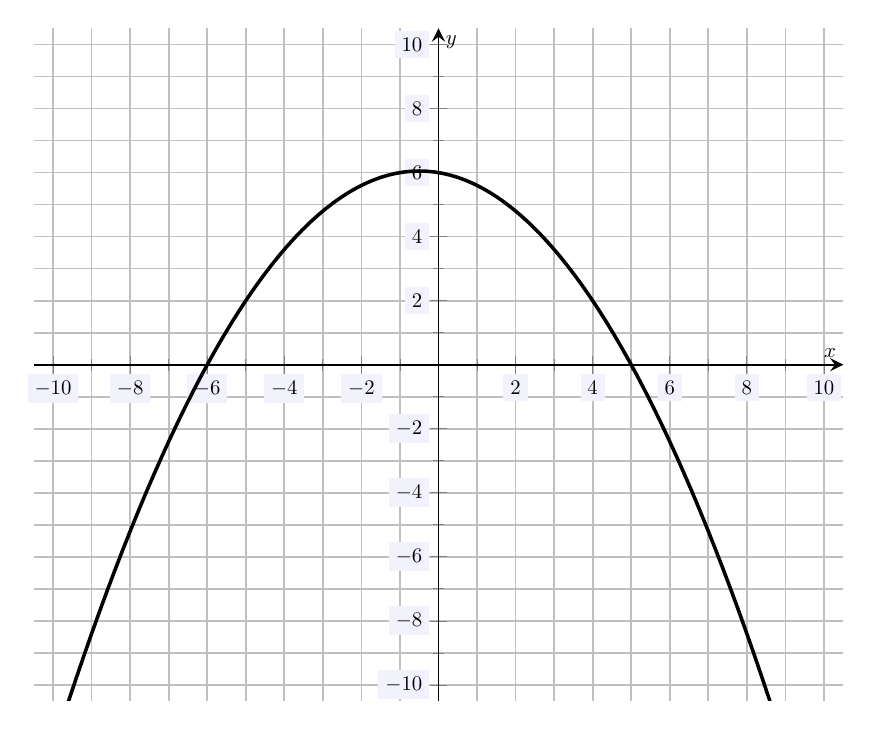
\begin{tikzpicture}[scale=1.5,every node/.style={scale=0.5}]
	\begin{axis}[
	grid=both,
	axis lines=middle,
	ticklabel style={fill=blue!5!white},
	xmin= -10.5, xmax=10.5,
	ymin= -10.5, ymax=10.5,
	xtick={-10,-8,-6,-4,-2,0,2,4,6,8,10},
	ytick={-10,-8,-6,-4,-2,0,2,4,6,8,10},
	minor tick = {-10,-9,...,10},
	xlabel=\(x\),ylabel=\(y\),
	]
	\addplot[line width=0.03cm,domain=-10:10,samples=100] ({x},{1/5*(-x^2 - x + 30)});
	\end{axis}
	\end{tikzpicture}
	}
	\] \pspace

\sol Let $f(x)$ be the plotted quadratic function. Observe that the quadratic function has $y$-intercept $(0, 6)$, i.e. $f(0)= 6$. We know that if a quadratic function $ax^2 + bx + c$ has roots, i.e. $x$-intercepts, $r_1, r_2$, the function factors as $a(x - r_1)(x - r_2)$. From the plot, we can see that $f(x)$ has roots $x= -6$ and $x= 5$. But then\dots
	\[
	f(x)= a(x - r_1)(x - r_2)= a \big(x - (-6) \big) (x - 5)= a(x + 6)(x - 5)
	\]
But we know that $f(0)= 6$. We then have\dots
	\[
	\begin{gathered}
	f(x)= a(x + 6)(x - 5) \\[0.3cm]
	f(0)= a(0 + 6)(0 - 5) \\[0.3cm]
	6= a(6)(-5) \\[0.3cm]
	6= -30a \\[0.3cm]
	a= -\dfrac{1}{5}
	\end{gathered}
	\]
Therefore, we know that\dots
	\[
	f(x)= -\dfrac{1}{5} \, (x + 6)(x - 5)
	\]



% Question 7
\newpage
\question[10] Without using a calculator and showing all your work, find the exact solution(s) to the following equation:
	\[
	x(x + 3)= 18
	\] \pspace

\sol Using factoring, we have\dots
	\[
	\begin{gathered}
	x(x + 3)= 18 \\[0.3cm]
	x^2 + 3x= 18 \\[0.3cm]
	x^2 + 3x - 18= 0 \\[0.3cm]
	(x + 6)(x - 3)= 0
	\end{gathered}
	\]
But then either $x + 6= 0$, which implies $x= -6$, or $x - 3= 0$, which implies $x= 3$. \pspace

Using the quadratic equation, we have\dots
	\[
	\begin{gathered}
	x(x + 3)= 18 \\[0.3cm]
	x^2 + 3x= 18 \\[0.3cm]
	x^2 + 3x - 18= 0 
	\end{gathered}
	\]
We then seek the roots of $x^2 + 3x - 18$, which has $a= 1$, $b= 3$, and $c= -18$. But the quadratic equation gives\dots
	\[
	\begin{aligned}
	x&= \dfrac{-b \pm \sqrt{b^2 - 4ac}}{2a} \\[0.3cm]
	&= \dfrac{-3 \pm \sqrt{3^2 - 4(1)(-18)}}{2(1)} \\[0.3cm]
	&= \dfrac{-3 \pm \sqrt{9 + 72}}{2} \\[0.3cm]
	&= \dfrac{-3 \pm \sqrt{81}}{2} \\[0.3cm]
	&= \dfrac{-3 \pm 9}{2}
	\end{aligned}
	\]
Therefore, either $x= \frac{-3 - 9}{2}= \frac{-12}{2}= -6$ or $x= \frac{-3 + 9}{2}= \frac{6}{2}= 3$. 



% Question 8
\newpage
\question[10] Without using a calculator and showing all your work, find the exact solution(s) to the following equation by using the quadratic formula:
	\[
	\dfrac{5x - 1}{x}= \dfrac{6x}{x - 1}
	\] \pspace

\sol We have\dots
	\[
	\begin{gathered}
	\dfrac{5x - 1}{x}= \dfrac{6x}{x - 1} \\[0.3cm]
	6x^2= (5x - 1)(x - 1) \\[0.3cm]
	6x^2= 5x^2 - 5x - x + 1 \\[0.3cm]
	6x^2= 5x^2 - 6x + 1 \\[0.3cm]
	x^2 + 6x - 1= 0
	\end{gathered}
	\]
The quadratic function $x^2 + 6x - 1$ has $a= 1$, $b= 6$, and $c= -1$. Observe the discriminant of this quadratic function is $b^2 - 4ac= 6^2 - 4(1)(-1)= 36 + 4= 40$, which is not a perfect square. Therefore, this polynomial does not factor `nicely' over the integers or rationals. Therefore, we find the solutions using the quadratic formula:
	\[
	\begin{aligned}
	x&= \dfrac{-b \pm \sqrt{b^2 - 4ac}}{2a} \\[0.3cm]
	&= \dfrac{-6 \pm \sqrt{6^2 - 4(1)(-1)}}{2(1)} \\[0.3cm]
	&= \dfrac{-6 \pm \sqrt{36 + 4}}{2} \\[0.3cm]
	&= \dfrac{-6 \pm \sqrt{40}}{2} \\[0.3cm]
	&= \dfrac{-6 \pm \sqrt{4 \cdot 10}}{2} \\[0.3cm]
	&= \dfrac{-6 \pm 2 \sqrt{10}}{2} \\[0.3cm]
	&= -3 \pm \sqrt{10}
	\end{aligned}
	\]



% Question 9
\newpage
\question[10] Consider the polynomial $p(x)= 9x^3 (x + 1) (x - 3)^2 (x + 6)^4 (x - 7)^9$.
	\begin{enumerate}[(a)]
	\item Find the degree of $p(x)$. 
	\item How many \textit{distinct} roots does $p(x)$ have?
	\item Find the roots of $p(x)$ along with their multiplicities. 
	\item Do the `ends' of $p(x)$ `point' in the same direction or opposite? Explain. 
	\item Does $p(x)$ have a maximum, minimum, both, or neither?
	\end{enumerate} \pspace

\sol 
\begin{enumerate}[(a)]
\item Recall a polynomial of the form $a(x - r_1)^{a_1} (x - r_2)^{a_2} \cdots (x - r_k)^{a_k}$ has degree $a_1 + a_2 + \cdots + a_k$, where $a_i > 0$ are integers for all $i$ and $a \neq 0$. Writing $p(x)= 9x^3 (x + 1) (x - 3)^2 (x + 6)^4 (x - 7)^9= 9(x - 0)^3 (x + 1)^1 (x - 3)^2 (x + 6)^4 (x - 7)^9$, we see that $p(x)$ has degree $3 + 1 + 2 + 4 + 9= 19$. \pspace

\item The roots of $p(x)$ are solutions to $9x^3 (x + 1) (x - 3)^2 (x + 6)^4 (x - 7)^9= 0$, which implies that $x^3= 0$, which implies $x= 0$, or $x + 1= 0$, which implies $x= -1$, or $(x - 3)^2= 0$, which implies $x= 3$, or $(x + 6)^4= 0$, which implies $x= -6$, or $(x - 7)^9= 0$, which implies $x= 7$. Therefore, there are five distinct zeros for $p(x)$. \pspace

\item The roots of $a(x - r_1)^{a_1} (x - r_2)^{a_2} \cdots (x - r_k)^{a_k}$, where $a_i > 0$ are integers for all $i$ and $a \neq 0$, are $r_1, r_2, \ldots, r_k$ and are said to have multiplicity $a_1, a_2, \ldots, a_k$, respectively. Writing $p(x)= 9x^3 (x + 1) (x - 3)^2 (x + 6)^4 (x - 7)^9= 9(x - 0)^3 (x + 1)^1 (x - 3)^2 (x + 6)^4 (x - 7)^9$, we see that $x= 0$ has multiplicity $3$, $x= -1$ has multiplicity $1$, $x= 3$ has multiplicity $2$, $x= -6$ has multiplicity $4$, and $x= 7$ has multiplicity $9$. \par
	\begin{table}[ht]
	\centering
	\begin{tabular}{l||r|r|r|r|r}
	Root & $0$ & $-1$ & $3$ & $-6$ & $7$ \\ \hline
	Multiplicity & $3$ & $1$ & $2$ & $4$ & $9$
	\end{tabular}
	\end{table}

\item We know from (a) that the degree of $p(x)$ is $19$, which is odd. Therefore, the `ends' of $p(x)$ `point' in opposite directions. \pspace

\item We know from (a) that the degree of $p(x)$ is $19$, which is odd. Therefore, while there may be local maxima or minima, there are no global maxima or minima.  
\end{enumerate}



% Question 10
\newpage
\question[10] Find the equation of the polynomial $p(x)$ plotted below, if $\deg p(x)= 6$. 
	\[
	\fbox{
	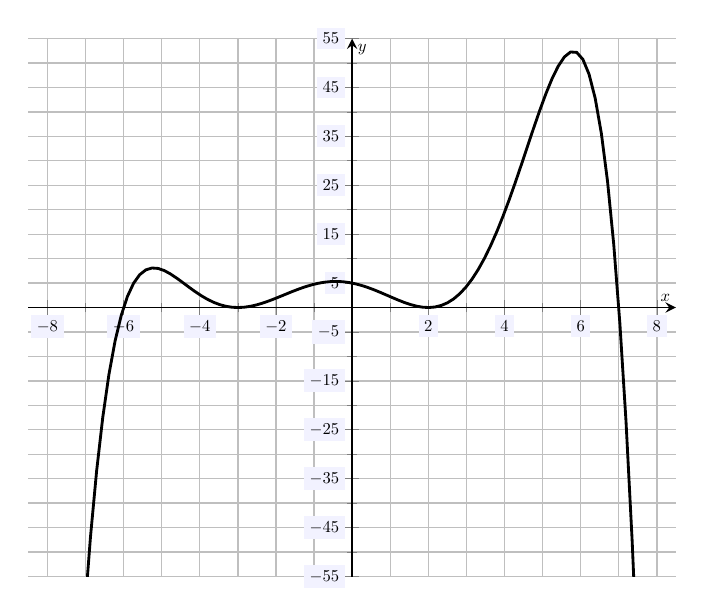
\begin{tikzpicture}[scale=1.2,every node/.style={scale=0.5}]
	\begin{axis}[
	grid=both,
	axis lines=middle,
	ticklabel style={fill=blue!5!white},
	xmin= -8.5, xmax=8.5,
	ymin= -55, ymax=55,
	xtick={-10,-8,-6,-4,-2,0,2,4,6,8,10},
	ytick={-55,-45,...,55},
%	minor tick = {-50,-40,...,50},
	minor x tick num = 1,
	minor y tick num = 1,
	xlabel=\(x\),ylabel=\(y\),
	]
	\addplot[line width=0.03cm,domain=-8:8,samples=100] ({x},{-5/1512*(x + 6)*(x + 3)^2*(x - 2)^2*(x - 7)});
	\end{axis}
	\end{tikzpicture}
	}
	\] 

\sol From the Fundamental Theorem of Algebra, we know the polynomial $p(x)$ factors as $p(x)= a(x - r_1)^{a_1} (x - r_2)^{a_2} \cdots (x - r_k)^{a_k}$, where $a_i > 0$ are integers for all $i$ and $a \neq 0$, then we know the degree of $p(x)$ is $a_1 + a_2 + \cdots + a_k$ and the roots of $p(x)$ are $r_1, r_2, \ldots, r_k$ with multiplicity $a_1, a_2, \ldots, a_k$, respectively. From the plot of $p(x)$, we see roots of $p(x)$ are $x= -6, -3, 2, 7$. \pspace

Therefore, we know that $p(x)$ has the form\dots
	\[
	p(x)= a \big(x - (-6) \big)^{a_1} \big(x - (-3) \big)^{a_2} (x - 2)^{a_3} (x - 7)^{a_4}= a (x + 6)^{a_1} (x + 3)^{a_2} (x - 2)^{a_3} (x - 7)^{a_4}
	\]
Because the degree of $p(x)$ is $6$, we know that $a_1 + a_2 + a_3 + a_4= 6$. We also know that if $p(x)$ `crosses' the $x$-axis at a root that root has odd multiplicity, and if $p(x)$ is `tangent' to the $x$-axis at a root that root has even multiplicity. From the plot of $p(x)$, we see that $x= -6$ and $x= 7$ have odd multiplicity and $x= -3$ and $x= 2$ have even multiplicity. Therefore, $a_1, a_4 \in \{ 1, 3, 5, \ldots \}$ and $a_2, a_3 \in \{ 2, 4, 6, \ldots \}$. But then $6= a_1 + a_2 + a_3 + a_4 \geq 1 + 2 + 2 + 1= 6$. But then this forces
	\[
	p(x)= a (x + 6)^{a_1} (x + 3)^{a_2} (x - 2)^{a_3} (x - 7)^{a_4}= a (x + 6) (x + 3)^2 (x - 2)^2 (x - 7)
	\] \pspace

Finally, we see that $p(x)$ has $y$-intercept $(0, 5)$, i.e. $p(0)= 5$. Then\dots
	\[
	\begin{gathered}
	p(x)= a (x + 6) (x + 3)^2 (x - 2)^2 (x - 7) \\
	p(0)= a (0 + 6) (0 + 3)^2 (0 - 2)^2 (0 - 7) \\
	5= -1512a \\
	a= -\dfrac{5}{1512}
	\end{gathered}
	\]
Therefore, 
	\[
	p(x)= -\dfrac{5}{1512} \, (x + 6) (x + 3)^2 (x - 2)^2 (x - 7)
	\]


\end{questions}
\end{document}